% Copyright 2004 by Till Tantau <tantau@users.sourceforge.net>.
%
% In principle, this file can be redistributed and/or modified under
% the terms of the GNU Public License, version 2.
%
% However, this file is supposed to be a template to be modified
% for your own needs. For this reason, if you use this file as a
% template and not specifically distribute it as part of a another
% package/program, I grant the extra permission to freely copy and
% modify this file as you see fit and even to delete this copyright
% notice. 

\documentclass{beamer}
\usepackage{graphicx}
\usepackage{multimedia}
\usepackage{caption}
\usepackage{subcaption}
\usepackage{media9}

\usepackage{chngcntr}
% There are many different themes available for Beamer. A comprehensive
% list with examples is given here:
% http://deic.uab.es/~iblanes/beamer_gallery/index_by_theme.html
% You can uncomment the themes below if you would like to use a different
% one:
%\usetheme{AnnArbor}
%\usetheme{Antibes}
%\usetheme{Bergen}
%\usetheme{Berkeley}
%\usetheme{Berlin}
%\usetheme{Boadilla}
%\usetheme{boxes}
%usetheme{CambridgeUS}
%\usetheme{Copenhagen}
%\usetheme{Darmstadt}
%\usetheme{default}
\usetheme{Frankfurt}
%\usetheme{Goettingen}
%\usetheme{Hannover}
%\usetheme{Ilmenau}
%\usetheme{JuanLesPins}
%\usetheme{Luebeck}
%\usetheme{Madrid}
%\usetheme{Malmoe}
%\usetheme{Marburg}
%\usetheme{Montpellier}
%\usetheme{PaloAlto}
%\usetheme{Pittsburgh}
%\usetheme{Rochester}
%\usetheme{Singapore}
%\usetheme{Szeged}
%\usetheme{Warsaw}

\title{Particle Aggregation Phenomena}

% A subtitle is optional and this may be deleted
\subtitle{Fractals and more!}

\author{ Gowtham Kuntumalla \and 140100091 \\ Kiran Ahire \and \and \and \and \and  15I120007 \\ Sukanya Kudva \and \and \and   160260026 \\  Aditya Venkatraman \and  16B030029 }
% - Give the names in the same order as the appear in the paper.
% - Use the \inst{?} command only if the authors have different
%   affiliation.

% - Use the \inst command only if there are several affiliations.
% - Keep it simple, no one is interested in your street address.

\date{PH 542 - Nonlinear Dynamics \\ Aug 30, 2017}
% - Either use conference name or its abbreviation.
% - Not really informative to the audience, more for people (including
%   yourself) who are reading the slides online

\subject{Theoretical Computer Science}
% This is only inserted into the PDF information catalog. Can be left
% out. 

% If you have a file called "university-logo-filename.xxx", where xxx
% is a graphic format that can be processed by latex or pdflatex,
% resp., then you can add a logo as follows:

% \pgfdeclareimage[height=0.5cm]{university-logo}{university-logo-filename}
% \logo{\pgfuseimage{university-logo}}


% Delete this, if you do not want the table of contents to pop up at
% the beginning of each subsection:
%\AtBeginSubsection[]
%{
 % \begin{frame}<beamer>{Outline}
  %  \tableofcontents[currentsection,currentsubsection]
 % \end{frame}
%}

% Let's get started
\begin{document}

\begin{frame}
  \titlepage
\end{frame}

\begin{frame}{Acknowledgements}
  \begin{itemize}
  \item {\emph{PhD Dissertation}, William Heinson, 2015}
  \item {\emph{The sol to gel transition in irreversible particulate systems}, C. M. Sorensen and A. Chakrabarti, Soft Matter, 2011, 7, 2284–2296}
  \item{\emph{Kinetic Percolation}, William Heinson et al, 2017 }
  % You might wish to add the option [pausesections]
  \item {Few images from Google image search. It will be mentioned in the presentation.}
  \item{Wikipedia articles for key concepts}
  \item{Credit for other work is given in the slides itself}
  \end{itemize}
\end{frame}

\begin{frame}{Outline}
  \tableofcontents
  % You might wish to add the option [pausesections]
\end{frame}

% Section and subsections will appear in the presentation overview
% and table of contents.
\section{Introduction}

\subsection{Why this topic?}

\begin{frame}{Why this topic?}
  Particle aggregation is a widely observed phenomenon in many seemingly unrelated fields. \\ 
  \vspace{15pt}
  
   Application areas 
  \begin{itemize}
      \item{
      Climate models- Very important in Aerosol science
      }
      \item{
      Condensation of stardust
      }
      \item{
      Colloidal particle dynamics
      }
      \item{
      Sol-Gel Transition
      }
      \item{
      Formation of River Delta
      }
      \item{
      Cheese Making :)
      }
      \item{
      Coagulation of blood and more!
      }
  \end{itemize}
\end{frame}

%-----------------------------END OF FRAME--------------------------------%

\subsection{Prerequisites}

% You can reveal the parts of a slide one at a time
% with the \pause command:
\begin{frame}{Types of Aggregation Models}
  \begin{itemize}
  \item {
    Diffusion based Models - (Stochastic)
  }
  \item {
   Ballistic motion based Models  - (Deterministic, except for initial random motions)
  }
  \item{
    Reaction Limited Model - (Slower version of DA with slight changes in thermodynamic interactions)
  }
  \end{itemize}
If we look at each model, One thing is common i.e. the way we describe the dynamically formed clusters - \alert{Fractals} \\
\vspace{10pt}
Fractals have very important implications in the fields of both reversible and irreversible aggregation. The equations involved are usually very complex and many factors simultaneously affect the process.
\end{frame} 
%-----------------------------END OF FRAME--------------------------------%

\begin{frame}{Langrangian vs Eulerian Perspective}

    Langrangian : \\ Viewing the simulation box from a single particle's point of view. i.e. It will be in a frame of reference where it is at rest.
    \begin{itemize}
        \item{
        Cluster-Monomer aggregation as in BA, DLA, RLA }
    \end{itemize}\\
    \vspace{20pt}
    Eulerian : \\ Viewing the simulation box from outside the box
    \begin{itemize}
        \item{
        Cluster-Cluster Aggregation as in BLCA, DLCA, RLCA}
    \end{itemize}
\end{frame}
%-----------------------------END OF FRAME--------------------------------%


\begin{frame}{Scaling Law}
The compact equation (\ref{scaling_eqn}) is known as the Scaling equation for aggregates which gives compact information about aggregates or clusters or agglomerates.

\begin{block}{Equation}
    \begin{equation} \label{scaling_eqn}
    N = k_o(Rg/a)^{D_f}
    \end{equation}
Where,
    \begin{itemize}
    \item {Df = Fractal dimension} % How effectively space is filled
    \item {ko = Prefactor Info about shape }
    \item {N = Number of monomer units in cluster}
    \item {Rg = Radius of gyration, a= Monomer radius}
   
    \end{itemize}
\end{block}
  
\end{frame}

%-----------------------------END OF FRAME--------------------------------%
\begin{frame}{General notion of Fractal dimension (Df)}
This is a 2D projection of 3D aggregates. 
    \begin{figure}[h]
        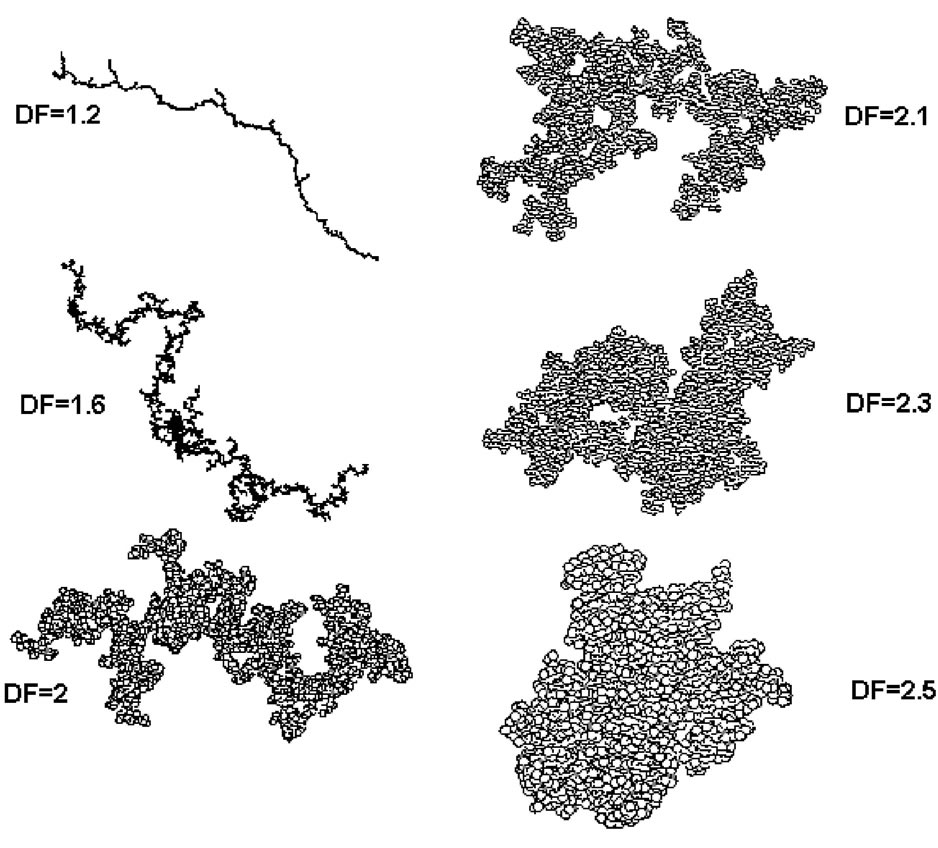
\includegraphics[scale=0.30]{diff_DF.jpg}
        % source http://file.scirp.org/Html/5-8301659/e57b4002-679c-4a89-a4db-67515b8b06b2.jpg
       \footnote{Source- DOI:10.4236/ns.2012.46052 }
    \end{figure}  
\end{frame}

%-----------------------------END OF FRAME--------------------------------%

\subsection{Basic types}



\begin{frame}{Diffusion Models}
  \begin{itemize}
  \item {Follow Brownian dynamics. Also heavier particles move slower}
      \item {There are two types: }
      \begin{enumerate}
          \item Diffusion limited monomer-cluster aggregation (DLA). Eg: Zinc ions in electrolyte near electrodes, Coral growth, Coalescing of smoke and dust.  
          \item Diffusion limited cluster-cluster aggregation (DLCA) Eg: Developed from DLA and works well for colloidal aggregation. Agrees with theory (\alert{${D_f}$=1.78}in 3D and 1.44 in 2D).
      \end{enumerate}
 
      \begin{figure}
\centering
\begin{minipage}{.5\textwidth}
  \centering
  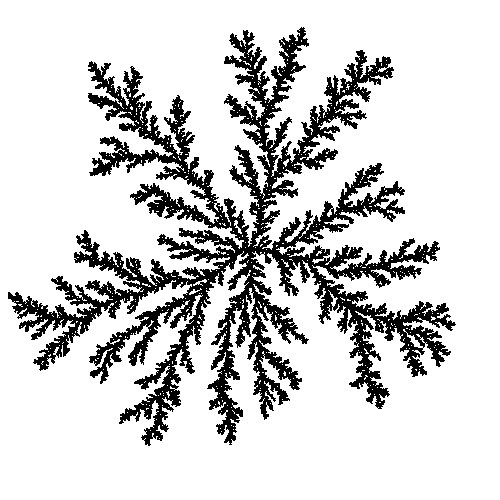
\includegraphics[width=.55\linewidth]{DLA.jpg}
  \captionof{figure}{DLA}
  \label{fig1:}
\end{minipage}%
\begin{minipage}{.5\textwidth}
  \centering
  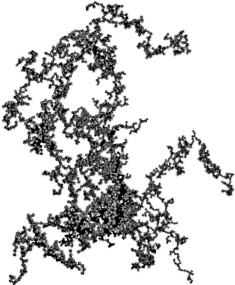
\includegraphics[width=.45\linewidth]{DLCA.jpg}
  \captionof{figure}{DLCA}
  \label{fig2:}
\end{minipage}
\end{figure}
     % \begin{figure}[l]
      %  \includegraphics[scale=0.25]{}
        % source http://file.scirp.org/Html/5-8301659/e57b4002-679c-4a89-a4db-67515b8b06b2.jpg
    %   \end{figure} 
  \end{itemize}
\end{frame}

%-----------------------------END OF FRAME--------------------------------%

\begin{frame}{Growth Kinetics Equation}
Growth Kinetics in cluster-cluster aggregation models is described by the Smoluchowski equation (\ref{smol_eqn}).
\begin{block}{Smoluchowski Equation}
    \begin{equation} \label{smol_eqn}
    \frac{dn_N}{dt} = \sum_{i=1}^{N-1} {K(i,N-i) n_i n_{N-i}} - n_N \sum_{i=1}^{\infty} {K(i,N)n_i}
    \end{equation}
\end{block}
Here ${n_i}$ is the number of clusters of size i. The kinetic state of the system is capture in the \alert{kernel K(i,j)}, which is dependent on the present state of the system. i.e \alert{time dependence}.\\ 

\emph{Thus \alert{Non linearity} is introduced into the system.}

% Aside: Observe that it is similar to "Master equation" (taught in BB101 - Biology)

\end{frame}
%-----------------------------END OF FRAME--------------------------------%


\begin{frame}{Ballistic models}
\begin{itemize}
  \item {\alert{Deterministic} system. Occurs in very low pressure situation or large molecular regime .High Knudsen number($K_n$) compared to diffusion scenario.}
  % {https://en.wikipedia.org/wiki/Knudsen\_number}
  \begin{equation}
      K_n= \frac{\lambda}{L} 
  \end{equation}
   where $\lambda$ = mean free path, L = representative physical length scale 
      \item {There are two types:}
      \begin{enumerate}
          \item Ballistic limited monomer-cluster aggregation (BLA). Eg: Thin film growth by vapor deposition   
          \item Ballistic limited cluster-cluster aggregation (BLCA). Agrees with theory (\alert{${D_f}$=1.91} in 3D and 1.55 in 2D)
      \end{enumerate}
\end{itemize}     
\end{frame}
%-----------------------------END OF FRAME--------------------------------%

\begin{frame}{Comparison}
    \begin{itemize}
        \item Look at the comparison between clusters formed through the different paths  
         \begin{figure}[h]
        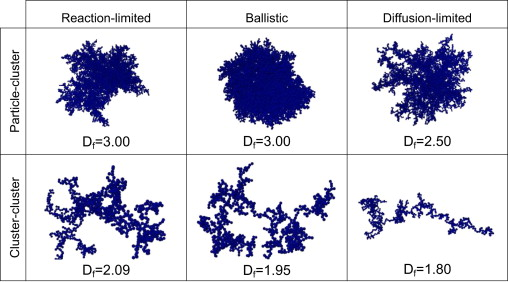
\includegraphics[scale=.85]{all_agg.jpg}
        \footnote{source: https://doi.org/10.1016/j.ces.2014.03.024}
    \end{figure} 
    \end{itemize}
\end{frame}
%-----------------------------END OF FRAME--------------------------------%

\section{Insights and Ideas}

\subsection{Simulations and remarkable observations!}

\begin{frame}{Time for simulations}
\begin{itemize}
    

\item Observe the following simulations done by us. The python code required for simulating it was relatively simple.
\item Parameters such as velocity of motion and number of particles in the system, etc affect the dynamics of the system.
\item Transitions from one mode to another in the same simulation system are seen!
\end{itemize}
\end{frame}
%-----------------------------END OF FRAME--------------------------------%
\subsection{What's new?}
\begin{frame} {Chaos in ballistic aggregation ?}
Something to ponder over.
\begin{itemize}
\item {In ballistic motion, We are sure of the path each  particle takes after every collision} 
\item {Does this mean the system is deterministic ?}
\item {Does slight change in initial conditions cause irreversible loss in predictability (subtly mentioning chaos)?}
\end{itemize}
\pause
Not all fractals are made same. There are self similar fractals, self affine fractals. (different $D_f$ along different directions). \\
\vspace{15pt}
\pause 
If fractal self similarity is necessary for chaos, Ballistic motion produced fractals are self affine. Hence we reject the notion of chaos here.  

\end{frame}
%-----------------------------END OF FRAME--------------------------------%

%\begin{frame}{Simulation movies that we created}

%\begin{frame}{remote (YouTube player)}

%\includemedia[
  %width=0.4\linewidth,
  %totalheight=0.225\linewidth,
  %activate=pageopen]
 %{\fbox{Click!}}{https://www.youtube.com/v/3QSyZV_4kCU}

%\begin{frame}

%\movie[label=show3,width=1.0\textwidth,poster     ,autostart,showcontrols,loop] 
 %{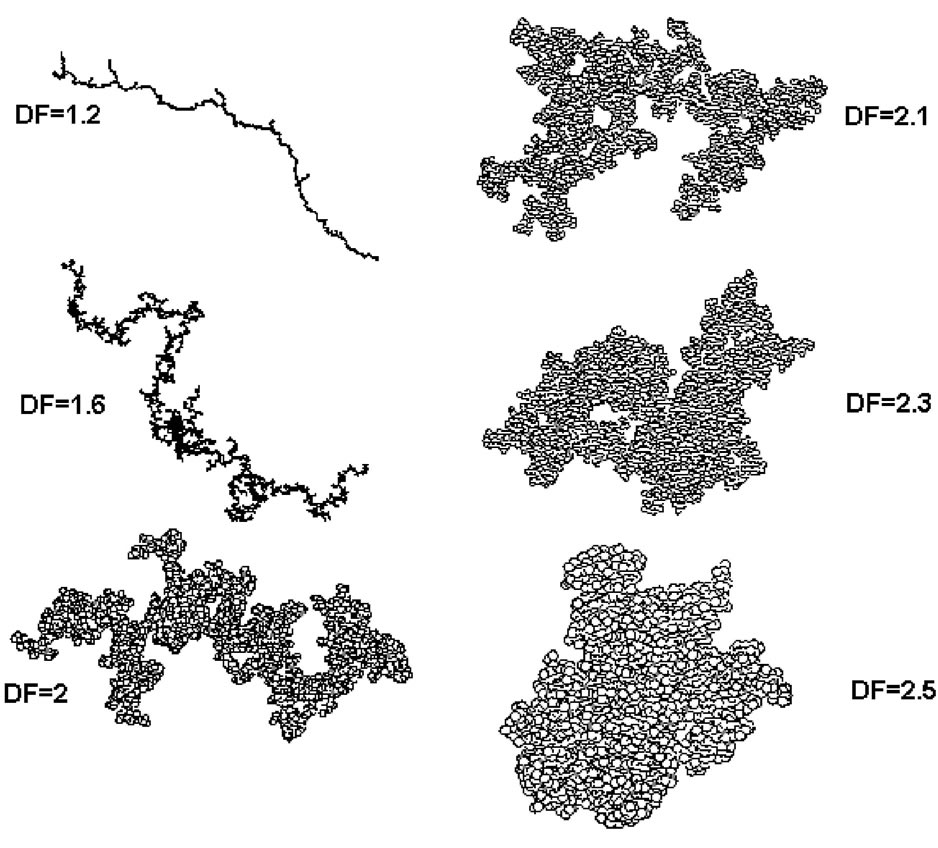
\includegraphics[width=.8\textwidth]{diff_DF.jpg}}{3D-Diffusion-Limited-Aggregation.mp4}
 
%\end{frame}

%-----------------------------END OF FRAME--------------------------------%

\section{The Sol-Gel transition}
   \begin{frame}{The Sol-Gel transition-1}
     \begin{itemize}
       \item Progression of events is as follows
    \end{itemize}
    \begin{figure}
        \centering
        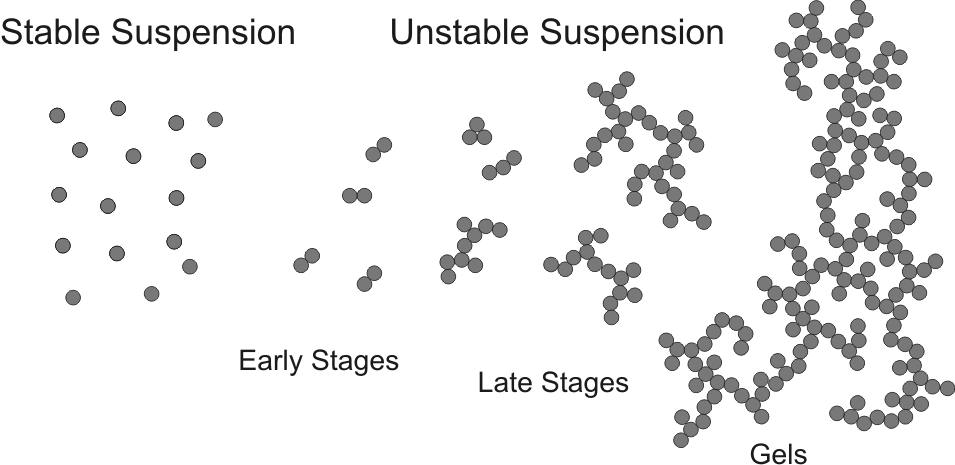
\includegraphics[scale=0.55]{gelation.png}
        \caption{Stable vs. Unstable systems}
        \label{fig:my_label}
    \end{figure}
    \end{frame}

%-----------------------------END OF FRAME--------------------------------%

\begin{frame}{The Sol-Gel transition-2}
     \begin{itemize}
      \item Compare this with the scaling equation mentioned earlier
    \end{itemize}
    \begin{figure}
        \centering
        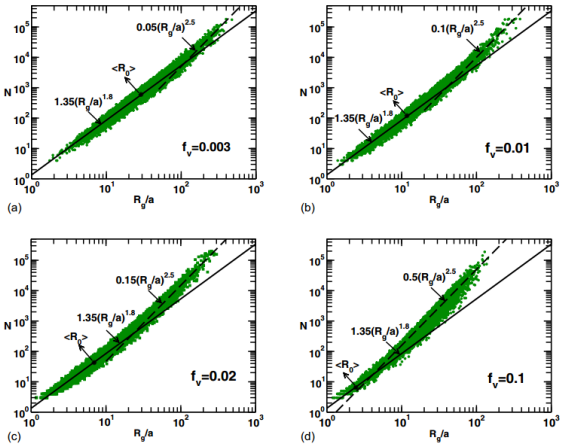
\includegraphics[scale=0.55]{Df-variation.png}
        \caption{Look at how Df (slope of line) varies}
        \label{Df-var}
    \end{figure}
    \end{frame}


% Placing a * after \section means it will not show in the
% outline or table of contents.
\section{Summary}

\begin{frame}{Summary}
  \begin{itemize}
  \item To stress the fact that fractals are really useful to explain things which seem too complex otherwise.
  \item
 We observe that in free molecular regime individual particles become irrelevant during this active, interactive process.   
   \item
  Random collision interactions between particles gives rise to something \alert{fundamental with a unique parameter} (ex: Df = 1.8 for 3D DLCA process) across multiple processes.
  \item Overall picture from a concatenated (in time) point of view makes more sense in stochastic simulations (fig \ref{Df-var})
   \end{itemize}
  
  \begin{itemize}
  \item
    Outlook
    \begin{itemize}
    \item
      Our Proposition is that given infinite amount of time any closed system will eventually attain fully gelled state (Tough to prove!).
    \item
    We think that ballistic does \alert{not} show chaos.
    \end{itemize}
    
  \end{itemize}
\end{frame}

%-----------------------------END OF FRAME--------------------------------%

\begin{frame}
\centering{Any more questions? \\} 

Thank you
\end{frame}
%-----------------------------END OF FRAME--------------------------------%



%-----------------------------END OF FRAME--------------------------------%
\end{document}


